% fanrisk - final report, ICTD 2026-27, IIT Delhi.
% Compiles with the ACM 'acmart' class (Overleaf has it built in). Without acmart.cls it falls back to a plain two-column
% article so a preview can still be built; the submitted version uses acmart.
\IfFileExists{acmart.cls}{\def\useacm{1}}{\def\useacm{0}}
\if1\useacm
  \documentclass[sigconf,nonacm]{acmart}
\else
  \documentclass[10pt,twocolumn]{article}
  \usepackage[margin=0.75in]{geometry}
  \usepackage{times}
  \usepackage[numbers,sort&compress]{natbib}
  \usepackage{hyperref}
  \newcommand{\affiliation}[1]{}
  \newcommand{\email}[1]{}
  \newcommand{\keywords}[1]{\gdef\kwtext{#1}}\def\kwtext{}
  \newenvironment{acks}{\section*{Acknowledgments}}{}
  \newsavebox{\absbox}
  \renewenvironment{abstract}{\global\setbox\absbox=\vbox\bgroup\hsize=0.86\textwidth\small\noindent\textbf{Abstract.}\ }{\egroup}
  \makeatletter
  \renewcommand{\maketitle}{\twocolumn[\begin{center}{\LARGE\bfseries\@title\par}\vspace{6pt}{\large Akhtar Hussain \quad Saharsh Laud\par}{\small Indian Institute of Technology Delhi, New Delhi, India\par}\vspace{8pt}\usebox{\absbox}\par\vspace{4pt}\parbox{0.86\textwidth}{\small\textbf{Keywords:} \kwtext}\vspace{10pt}\end{center}]}
  \makeatother
\fi
\usepackage{booktabs}
\usepackage{graphicx}
\usepackage{amsmath}
\usepackage{xcolor}
\graphicspath{{figures/}}

\title{Scenario-Driven Flash-Flood Simulation for Ladakh's Alluvial-Fan Settlements: From Automated Fan Identification and AHP Risk Mapping to HEC-RAS 2D, Validated on Leh 2010}

\author{Akhtar Hussain}
\affiliation{%
  \institution{Indian Institute of Technology Delhi}
  \city{New Delhi}
  \country{India}}
\email{mcs262729@cse.iitd.ac.in}

\author{Saharsh Laud}
\affiliation{%
  \institution{Indian Institute of Technology Delhi}
  \city{New Delhi}
  \country{India}}
\email{mcs242002@cse.iitd.ac.in}

\begin{document}

\begin{abstract}
Settlements in Ladakh and across the Himalaya are built on alluvial fans, at the mouths of steep catchments where a short cloudburst turns into a flash flood or debris flow. The 2010 Leh cloudburst killed more than 250 people. Most of the deaths were on two fans, while the nearest rain gauge logged 12.8\,mm that day. District authorities have no fan-scale hazard maps and no hydraulic modelling capacity, and cloudbursts this local cannot yet be forecast.

We present \texttt{fanrisk}, an open Python pipeline that maps, for a given storm scenario, which fans, which parts of each fan and which buildings are in danger. It starts from a freely available 30\,m DEM, identifies fans and their catchments, ranks them with a two-level Analytic Hierarchy Process (AHP), builds and runs a HEC-RAS 2D model of the main flood path without the graphical interface, and overlays buildings, roads and critical facilities.

Against the 2010 flood footprint at Choglamsar, the AHP risk map reaches an AUC of 0.85 (POD 0.59, FAR 0.16). The HEC-RAS model reaches an AUC of 0.77 and reproduces the observed depth at the gauged Sabu section within 3\%. The AHP result is stable across 423 random perturbations of the expert judgements (AUC 0.82--0.85). The hydraulic result is stable across Manning's $n$ from 0.04 to 0.08 (AUC 0.76--0.77). In the hindcast, 541 present-day buildings are flooded 0.3\,m or deeper, 200 of them in the extreme hazard class.

Run without any tuning on the 2025 Dharali debris flow (Uttarakhand), the pipeline does not find the fan on its own. Given one manual apex, it measures the catchment within 8\% of the published value, classifies the event correctly as a debris flow, and marks the area around the deposit as high risk. To check that nothing in the tool is tuned to Leh, we also ran the full chain, HEC-RAS included, on the 2013 Kedarnath flood with default settings and the tool's own storm hydrograph. The model runs stably in a new map zone and sends the flood through the town at 1.6--2.6\,m and 5--6\,m/s. Of the cells HEC-RAS rates significant or extreme, 89\% are high risk on the AHP map; the AHP's AUC against the simulated flood is 0.73--0.75, against 0.83--0.86 at Leh. The test exposed one hidden Leh assumption in the code, which we fixed. We close with an impact-assessment design for the District Disaster Management Authority, panchayats and households, and release the tool, data and results on GitHub.
\end{abstract}

\keywords{flash flood, alluvial fan, cloudburst, AHP, HEC-RAS 2D, scenario mapping, Ladakh, Himalaya, reproducibility, ICTD}

\maketitle

% =====================================================================================
\section{Introduction}
Ladakh lies in the rain shadow of the Great Himalaya, but aridity does not remove flood risk. On 4--6 August 2010 a cloudburst over Leh produced flash floods and debris flows. More than 250 people died, 1,749 houses were destroyed across 52 villages, and the region was cut off \cite{thayyen2013}. Reconstructed rainfall reached about 209--320\,mm in under twelve minutes over sub-kilometre areas, while the nearest gauge recorded 12.8\,mm for the day \cite{thayyen2013}. The deaths concentrated on the Sabu--Choglamsar fan and the Leh town fan, the places where water and debris left a confined channel and spread over houses \cite{bhatt2011}.

The landform sequence is always the same: a steep catchment generates runoff and sediment, a feeder channel concentrates it, and an alluvial fan spreads it where people live. Regional susceptibility rasters blur this sequence \cite{negi2020,sharma2023}. Hydraulic models resolve it, but need terrain processing, a hand-built model and an engineer to run it, none of which a district office has.

We built \texttt{fanrisk} to close that gap for the people who make siting and evacuation decisions: the District Disaster Management Authority (DDMA), panchayats and residents. It asks, for a given storm: which fans, which parts of each fan, and which buildings are in danger, and how deep and fast will the water be? Our contributions are:
\begin{enumerate}
  \item An \textbf{automated chain from a DEM to validated maps}: fan and catchment identification, a two-level AHP that separates catchment source susceptibility from fan hazard and exposure, and a HEC-RAS 2D model fitted, run in batch and read back without the GUI (Section~\ref{sec:method}).
  \item \textbf{Validation against an observed flood}: a footprint and 648 damaged houses traced from satellite damage mapping of the 2010 event, scored with AUC, POD, FAR and CSI. This is supported by sensitivity tests on the AHP judgements, terrain conditioning and roughness, and a cross-check against published values (Section~\ref{sec:results}).
  \item \textbf{Transfer tests on two more events} in a different climate and valley type, with no tuning: Dharali 2025 (Section~\ref{sec:dharali}) and Kedarnath 2013, where the whole chain including HEC-RAS is run to test for bias toward Leh (Section~\ref{sec:kedarnath}). They report where the pipeline fails as well as where it works.
  \item An \textbf{exposure layer and a delivery format} for non-specialists, and an \textbf{impact-assessment design} with indicators and survey instruments (Section~\ref{sec:impact}).
\end{enumerate}
\textbf{How the project evolved.} The proposal (Assignment~1) framed a three-stage, fan-centred pipeline that would be driven by weather forecasts: identify the fans, map risk on them with AHP, and simulate the flood with HEC-RAS 2D. The first prototype (Assignment~2) did Stages~1 and~2 by hand, with QGIS-drawn fans and a Google Earth Engine AHP, and was not yet validated. The interim (Assignment~3) automated Stage~1, moved Stage~2 to absolute physical scales and ran a first, hand-built HEC-RAS model. It also showed that uniform rain under-predicts the 2010 Sabu peak by 61\%, because a cloudburst falls on part of a basin (Section~\ref{sec:limits}). This paper reports the final phase: the observed footprint, the routing fix, a fully automated HEC-RAS stage, sensitivity tests, exposure, two further events and the open release. Because of the 61\% result, the pipeline is \emph{scenario-driven}: it answers ``what if this storm or this flood arrives?'' and leaves cloudburst forecasting as future work.

The code, data, example runs and results are public at \url{https://github.com/SaharshLaud/fanrisk}.

% =====================================================================================
\section{Related Work}
\textbf{Fan identification.} Morphometric indices separate flood-prone from debris-flow-prone fans. The Melton ratio, catchment relief divided by the square root of catchment area, is the most used: below about 0.3 for floods, 0.3--0.6 for debris floods, above 0.6 for debris flows \cite{wilford2004,descally2010,santangelo2012}. Norini et al. delineate fans automatically from DEMs by finding apexes where channels leave confined terrain and growing radial cones \cite{norini2016}. Our Stage~1 follows that idea with a valley-mouth detector based on terrain openness.

\textbf{Multi-criteria susceptibility.} AHP weighted overlays are common for flash-flood and debris-flow susceptibility in data-scarce mountains \cite{saaty1980,negi2020,elsebaie2023,karkani2021}. They are rarely validated against an observed footprint, and their sensitivity to the expert judgements is rarely reported \cite{feizizadeh2014,chen2010}. Negi et al. report an AUC of 0.766 for rainfall-induced debris-flow zones in Ladakh--Nubra \cite{negi2020}, which we use as a regional benchmark.

\textbf{Coupling screening with hydraulics.} Several studies couple GIS multi-criteria maps with HEC-RAS simulations; Elsebaie et al., for example, check a GIS--AHP flood map against a 2D HEC-RAS model of the 2018 Wadi Al-Lith flood \cite{elsebaie2023}. In practice each model is built by hand for one reach. The open \texttt{ras-commander} library makes HEC-RAS scriptable \cite{rascommander}, which lets the hydraulic step become part of an automated pipeline.

\textbf{ICTD and early warning.} A people-centred early warning system has four elements: risk knowledge, monitoring and forecasting, dissemination, and preparedness to respond \cite{wmo2018}. Tools built for disaster agencies succeed or fail on whether officials and communities can read and act on them. We therefore design the evaluation around comprehension, decisions and harm, not only accuracy (Section~\ref{sec:impact}).

% =====================================================================================
\section{Study Areas and Data}
\textbf{Leh 2010 (validation).} The Leh DEM is Copernicus GLO-30 \cite{copdem}, reprojected to UTM 43N at 26.7\,m (909 $\times$ 781 cells). Observations come from two sources:
\begin{itemize}
  \item Thayyen et al. \cite{thayyen2013} provide the reconstructed Sabu hydrograph (peak 1,070\,m$^3$/s at 23\,min) and the flow at section ST1 (depth 5.2\,m, velocity 8.3\,m/s, $\pm$35\%).
  \item From Bhatt et al.'s damage map \cite{bhatt2011} we traced the severely affected area at Choglamsar (0.77\,km$^2$), 648 damaged houses and the window actually mapped. The figure was georeferenced to imagery by matching the stream line at a fixed scale (rms 17\,m).
\end{itemize}

\textbf{Dharali 2025 (transfer test).} On 5 August 2025 a debris flow from the Kheer Gad (Khirganga) buried Dharali village on its fan at the Bhagirathi confluence. At least 60 people died or went missing. Published values: catchment 17\,km$^2$, Melton ruggedness 0.8, deposit about 18--20\,ha (about 750 $\times$ 450\,m) \cite{kumar2026,isro2025}. The DEM was downloaded fresh by the tool (Copernicus GLO-30, two tiles).

\textbf{Kedarnath 2013 (bias test).} On 16--17 June 2013, 325\,mm of rain in 24\,h at Chorabari and the outburst of Chorabari Lake, 2\,km upstream, sent a flood and debris down the Mandakini through Kedarnath town (3,583\,m) to Gaurikund, 16\,km downstream. Both banks were washed away and thousands died. The Kedarnath valley covers about 67\,km$^2$, 23\% of it glaciated \cite{singh2015}. No flood footprint or measured depth is published for the town, so we use this event to test the pipeline's behaviour, not its accuracy.

\textbf{Exposure.} Buildings come from Microsoft Global ML Building Footprints (25,384 in the Leh study area) \cite{msbuildings}. OpenStreetMap lists only 805 buildings there, 17 of them inside the surveyed window, against 648 damaged houses in 2010. Roads (270\,km) and 29 critical facilities come from OpenStreetMap.

% =====================================================================================
\section{Method}\label{sec:method}
\begin{figure*}[t]
  \centering
  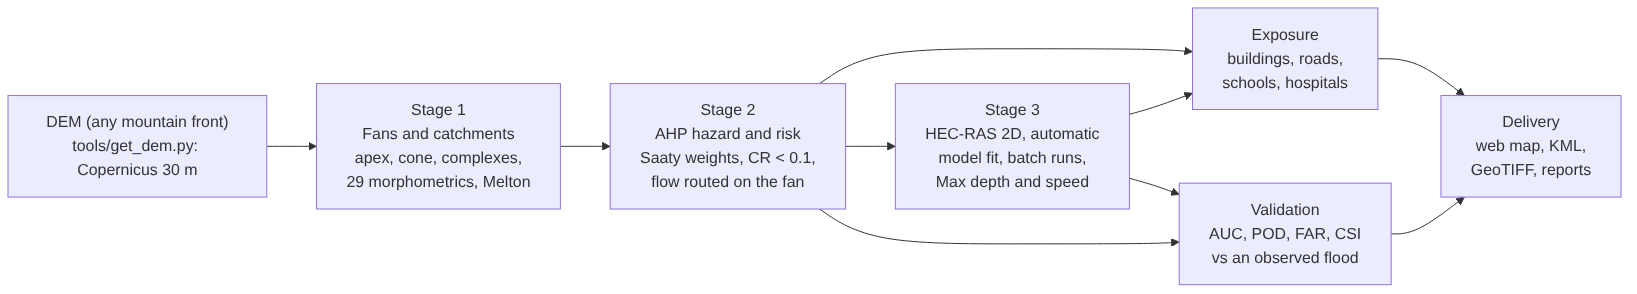
\includegraphics[width=\textwidth]{pipeline.png}
  \caption{The \texttt{fanrisk} pipeline. Each stage narrows the area and raises physical detail, so the expensive 2D solver only runs where the cheap stages say it matters.}
  \label{fig:pipeline}
\end{figure*}

Figure~\ref{fig:pipeline} shows the stages. Every number comes from four layers, each overriding the one before:
\begin{enumerate}
  \item method defaults;
  \item a region profile (arid, humid or generic mountain);
  \item the site file;
  \item an explicit override section.
\end{enumerate}
The run log lists every value that differs from the defaults and where it came from. Leh 2010 is stored as a validation case, never as a default.

\subsection{Stage 1: fans and catchments}
The DEM is sink-filled and flow is accumulated, and channels are cells draining more than 0.5\,km$^2$. An apex is the first channel cell where the terrain \emph{openness} reaches 90\% of its value 2\,km downstream. Openness is the number of 16 compass directions in which the terrain does not rise above 8$^\circ$ within 1\,km. The detector also requires that openness rose by at least 5 directions and reaches at least 8. From each apex a radial cone is grown on a channel-filled surface. Touching fans merge into complexes, and the full catchment of every feeder is delineated. Twenty-nine morphometric values are recorded per feeder, including the Melton ratio, which sets the flow type (breaks 0.3 and 0.6 \cite{wilford2004}).

Against hand-traced polygons the Sabu fan reaches an IoU of 0.86 and its catchment 0.96. The Sabu catchment is 62.4\,km$^2$, against 64.95\,km$^2$ published (\,$-4\%$). The same settings run unchanged on Trail Canyon, Death Valley.

\subsection{Stage 2: two-level AHP}
\begin{table*}[t]
  \caption{AHP criteria. Each criterion is scored from 0 to 1 on a fixed physical scale, so a score means the same on every fan and DEM. Weights are for Leh, where the two optional catchment layers were not supplied and the matrix was re-solved without them; flow accumulation and upstream area, the same quantity from a DEM, are merged.}
  \label{tab:ahp}
  \footnotesize
  \begin{tabular}{@{}llp{0.40\textwidth}lc@{}}
    \toprule
    AHP & Criterion & Why it matters & Scale (score 0 $\rightarrow$ 1) & Weight \\
    \midrule
    Catchment $C$ & Slope & Steep slopes shed rain fast and mobilise loose debris \cite{negi2020} & region range & 0.372 \\
     & Local relief ($\pm$500\,m) & Height difference gives flow energy; the basis of the Melton ratio \cite{wilford2004} & region range & 0.249 \\
     & Upstream area & A larger catchment collects more water & 0.5 $\rightarrow$ 100\,km$^2$ (log) & 0.307 \\
     & Ruggedness (TRI) & Jagged terrain supplies sediment \cite{riley1999} & region range & 0.073 \\
     & Historical rainfall (optional) & Wetter catchments flood more often & region range & -- \\
     & Bare or sparse ground (optional) & Bare rock and gravel give near-total runoff & region range & -- \\
    \midrule
    Fan $H$ & Inverse HAND & Ground barely above the channel is reached first \cite{nobre2011} & 10\,m $\rightarrow$ 0\,m above channel & 0.306 \\
     & Routed upstream area & Where the feeders' flow actually goes on the fan \cite{holmgren1994} & 0.05 $\rightarrow$ 100\,km$^2$ (log) & 0.295 \\
     & Fan slope & Steeper fans give faster, more forceful flow \cite{santangelo2012} & 0 $\rightarrow$ 10$^\circ$ & 0.212 \\
     & Local relief & Channel banks and rugged surroundings & 0 $\rightarrow$ 300\,m & 0.100 \\
     & Event rainfall (if given) & Local runoff on the fan & 0 $\rightarrow$ 100\,mm & 0.087 \\
    \bottomrule
  \end{tabular}
\end{table*}
Catchment source susceptibility $C$ (one value per feeder) and fan hazard $H$ (one value per cell) are scored separately (Table~\ref{tab:ahp}). Weights come from Saaty pairwise matrices on the 1--9 scale \cite{saaty1980}, judged by us from the literature and the physics of fan flooding, and solved by the principal eigenvector. The consistency ratios are 0.020 for the catchment matrix and 0.043 for the fan matrix, below the 0.10 limit. A low CR shows the judgements are self-consistent, not that they are right; that is tested against the 2010 flood and by perturbation (Section~\ref{sec:results}). Criteria without data are dropped and the matrix is re-solved, so the pipeline runs on a DEM alone.

The scale end-points are physical reference values fixed in Assignment~3, before the 2010 footprint was traced: 10\,m of HAND is about twice the largest credible flow depth (5.2\,m observed at Sabu); 10$^\circ$ is the steep end of alluvial-fan slopes; 100\,km$^2$ is the upper end of catchments that feed single fans (Sabu is 62\,km$^2$); 100\,mm is an extreme event for Ladakh. The earlier percentile scaling made a score depend on what else was in the map.

Exposure modifies hazard as $E = 0.5 + 0.5B$ with built-up density $B$ ($E = 1$ when no layer is given), so an empty but dangerous cell keeps half its hazard; risk is $R = H \cdot E$. Each feeder $i$ also gets its own scenario map, $H_i E (0.5 + 0.5C_i)(0.5 + 0.5T_i)$, where $T_i$ scales its peak flow for the given storm from 5 to 1,000\,m$^3$/s on a log scale; the worst case over feeders is reported per cell. Classes break at 0.2, 0.4, 0.55 and 0.7. Equal steps would leave the top class empty, because no cell scores high on every criterion at once; 0.7 marks about the top 1\% of fan cells on the test DEMs, the apex mouths and main flow paths. AUC is computed on the continuous score and does not depend on these breaks.

Flow from each feeder is routed across the fan by multiple-flow-direction routing \cite{holmgren1994}, with a run-out corridor to the trunk river. An early version routed on the channel-filled fan surface used for delineation. This spread the modelled flow away from the incised channel the 2010 flood followed. The pipeline now routes on the real DEM (Section~\ref{sec:routing}).

\subsection{Stage 3: HEC-RAS 2D without the GUI}
For the chosen feeder the pipeline writes a handoff package: clipped terrain, flow-area polygon, centreline, inflow and outflow lines, hydrographs and a nine-run scenario table (flow $\times$ 0.65, 1.0, 1.35 crossed with clear water, bulked and Bingham). The command \texttt{hecras fit} re-targets a bundled minimal HEC-RAS 7.0.2 project to this package. It sets:
\begin{itemize}
  \item the perimeter, with computation points at 15\,m;
  \item the boundary lines, with outflow friction slope 0.0055;
  \item the full shallow-water equations, since the flow is fast and supercritical;
  \item the projection and the terrain.
\end{itemize}
The inflow hydrograph is either an observed event (Leh: the reconstructed triangular hydrograph, 1,070\,m$^3$/s at 23\,min \cite{thayyen2013}) or built from a rain scenario with the SCS curve-number method: runoff from the curve number and antecedent moisture, time to peak from half the storm duration plus 0.6 times the Kirpich time of concentration, and peak $Q_p = 0.208\,A\,Q/T_p$ \cite{chow1988,kirpich1940}. The flow scales of $\pm$35\% follow the stated uncertainty of the observed peaks. Bulked runs divide the clear-water flow by $1 - C_v$, with $C_v$ = 0.25 for debris floods and 0.45 for debris flows, values at the cautious lower end of the standard sediment-concentration classes \cite{obrien1988}; Bingham runs are listed but need rheology that was never measured here.

A batch command then writes each hydrograph, runs HEC-RAS headless through \texttt{ras-commander} \cite{rascommander}, exports maximum depth and velocity, and scores the run. Where the HEC-RAS map export is unavailable, maximum maps are rebuilt from the results file. Against HEC-RAS's own maps of the same run, depth differs by 0.11\,m on average (wet-area IoU 0.79) and speed by 0.20\,m/s. Hazard follows the UK depth--velocity rating $HR = d(v + 0.5) + DF$, classed at 0.75, 1.25 and 2.5 (danger for some, most and all) \cite{fd2321}. We use a constant debris factor $DF = 0.5$; the guidance varies it from 0 to 1 with depth and land use, so hazard in built-up cells is if anything understated.

Two terrain and roughness choices are tested rather than assumed:
\begin{itemize}
  \item \textbf{Channel burn.} A 27\,m DEM is about as wide as the channel, so a 40\,m strip, about one to two cells, is lowered 0, 2 or 4\,m below the never-rising bed profile of the centreline. The depth is tested; the width is a fixed setting.
  \item \textbf{Roughness.} One Manning's $n$ is used for the whole area (0.06, within the 0.04--0.07 range for boulder mountain channels \cite{chow1959}), and 0.04 and 0.08 are tested.
\end{itemize}

\subsection{Exposure and validation}
Building centroids, road segments sampled every 10\,m, and facility points are classed by AHP risk, HEC-RAS hazard and the observed footprint.

Validation scores only cells inside the window that was surveyed. Footprint cells are positives and the rest of the window negatives. AHP cells not covered by any complex score 0, since leaving them out would flatter the map. We report:
\begin{itemize}
  \item AUC (Mann--Whitney);
  \item POD, FAR and CSI for the binary map (AHP high or above; HEC-RAS depth $\geq$ 0.3\,m);
  \item the share of damaged houses hit.
\end{itemize}

% =====================================================================================
\section{Results: Leh 2010}\label{sec:results}

\subsection{Routing on the real DEM}\label{sec:routing}
\begin{figure}[t]
  \centering
  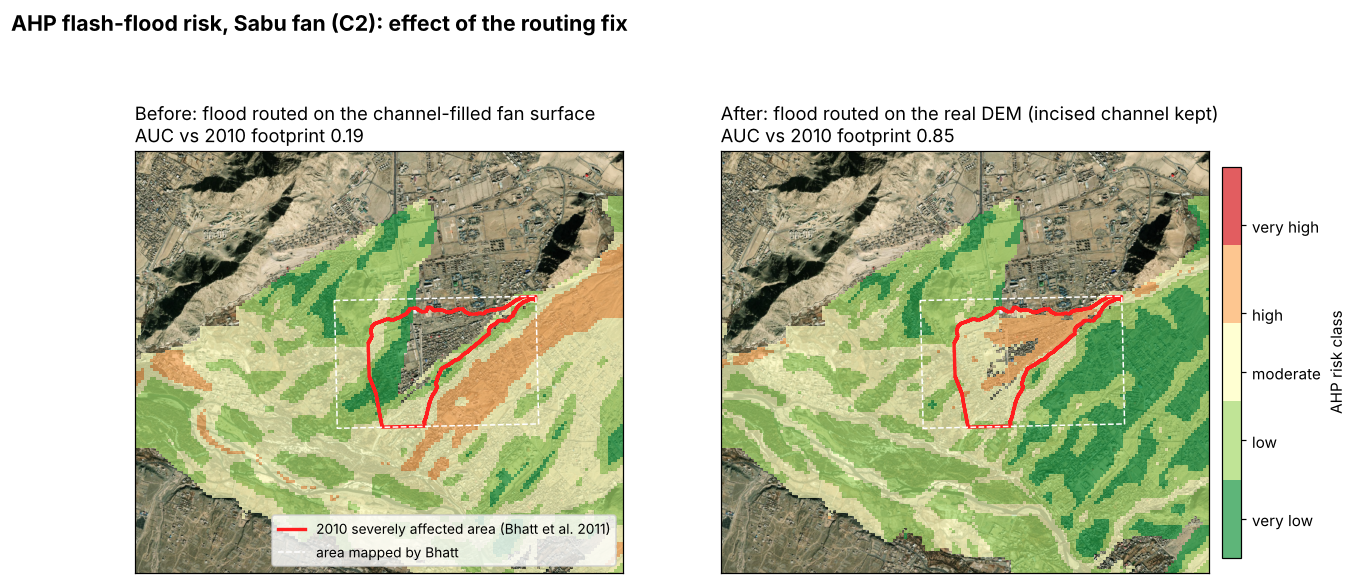
\includegraphics[width=\columnwidth]{ahp_routing_fix_before_after.png}
  \caption{AHP risk on the Sabu fan before and after routing on the real DEM. Red: 2010 severely affected area \cite{bhatt2011}; dashed: area mapped. AUC rises from 0.19 to 0.85. Imagery \copyright\ Esri.}
  \label{fig:routing}
\end{figure}
Routed on the channel-filled surface, the AHP map ranked the 2010 footprint \emph{below} its surroundings (AUC 0.19) and covered only 57\% of it. Routed on the real DEM, it reaches an AUC of 0.85, POD 0.59 and FAR 0.16, and covers 90\% (Figure~\ref{fig:routing}). Its agreement with HEC-RAS rises from an AUC of 0.59 to 0.81. Only blend weights of 0, 0.5 and 1 were tried; we chose 0 on physical grounds, not by tuning. One disagreement remains: AHP rates the first 1.2\,km of the Sabu channel moderate where HEC-RAS rates it extreme.

\subsection{Hydraulic model and terrain conditioning}
\begin{table}[t]
  \caption{HEC-RAS run R04 (1,070\,m$^3$/s, clear water) against the 2010 footprint and Sabu ST1 (observed 5.2\,m, 8.3\,m/s).}
  \label{tab:burn}
  \small
  \begin{tabular}{@{}lccccc@{}}
    \toprule
    Variant & AUC & POD & FAR & CSI & ST1 depth (m) \\
    \midrule
    No burn            & 0.706 & 0.54 & 0.43 & 0.39 & 4.53 \\
    \textbf{Burn 2\,m} & \textbf{0.770} & 0.51 & \textbf{0.34} & \textbf{0.40} & \textbf{5.04} \\
    Burn 4\,m          & 0.758 & 0.38 & 0.32 & 0.32 & 5.61 \\
    \midrule
    $n = 0.04$ (2\,m)  & 0.762 & 0.42 & 0.33 & 0.35 & 4.79 \\
    $n = 0.08$ (2\,m)  & 0.767 & 0.58 & 0.36 & 0.44 & 5.33 \\
    \bottomrule
  \end{tabular}
\end{table}
Burning the channel 2\,m into the terrain gives the best match (Table~\ref{tab:burn}, Figure~\ref{fig:burn}): AUC 0.77, FAR down from 0.43 to 0.34, and ST1 depth within 3\%. Speed at ST1 is 6.9\,m/s against 8.3\,m/s observed ($-17\%$), within the $\pm$35\% observation tolerance; the 27\,m terrain smooths the channel and slows the modelled flow. A 4\,m notch over-confines the flood (POD 0.38). This matches a Manning capacity estimate made before the runs: at the mean bed slope of 4.6\%, a 2\,m notch carries about 40\% of the peak, so the flood still spreads over the fan as in 2010, while a 4\,m notch carries about 120\%.

Roughness changes the flooded area by about $\pm$15\%. It leaves the ranking (AUC 0.76--0.77) and the extreme-hazard area (0.48--0.49\,km$^2$) almost unchanged. No single $n$ matches both depth and speed at ST1; all values lie within the $\pm$35\% observation tolerance. Jarrett found that $n$ rises with slope in high-gradient streams \cite{jarrett1984}, so values up to 0.08 are plausible here.

\begin{figure}[t]
  \centering
  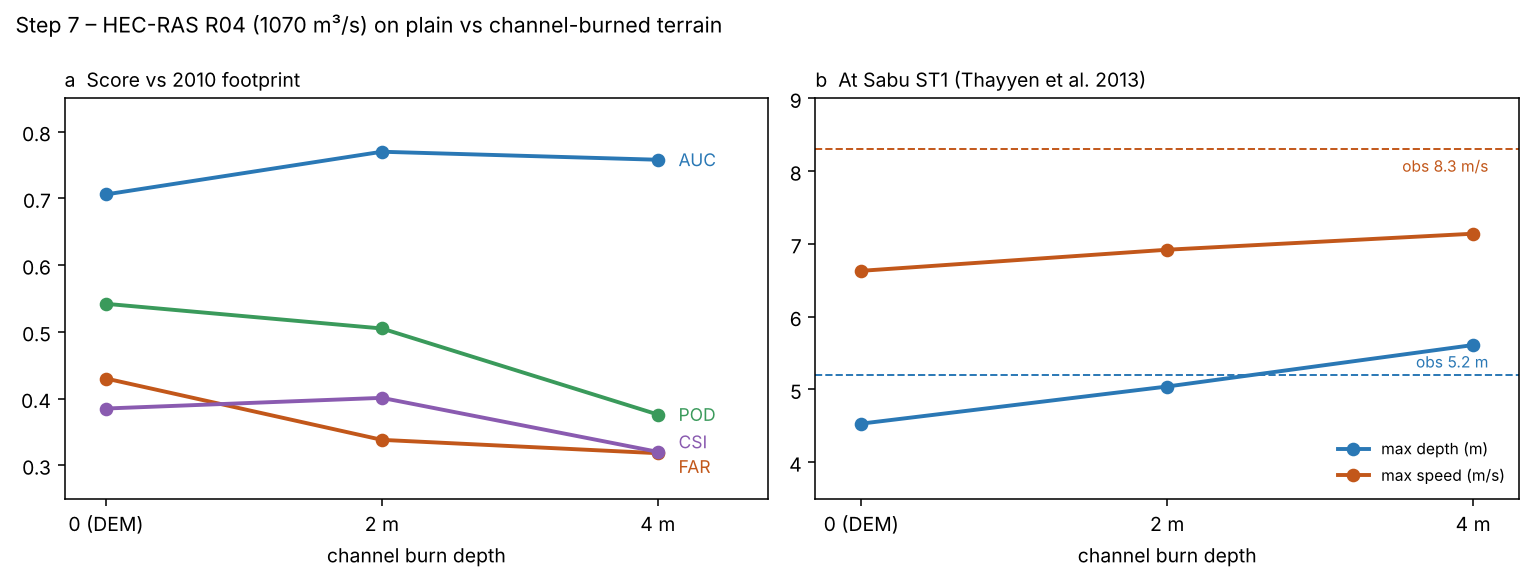
\includegraphics[width=\columnwidth]{channel_burn_results.png}
  \caption{Channel burn: skill against the 2010 footprint (a) and flow at Sabu ST1 (b).}
  \label{fig:burn}
\end{figure}

\subsection{Sensitivity of the AHP to expert judgement}
We perturbed every Saaty pairwise judgement by $\pm$1 or $\pm$2 steps and kept only samples with CR $\leq$ 0.10 (340 and 83 samples) \cite{feizizadeh2014}. We also scaled each fan weight from 0.5 to 1.5 with renormalisation \cite{chen2010}.
\begin{itemize}
  \item AUC against the footprint stays at 0.845--0.850 for $\pm$1 step, with a minimum of 0.824 for $\pm$2.
  \item Every sample beats the regional benchmark of 0.766 \cite{negi2020}, and nearly all lie in the 0.8--0.9 ``excellent'' band \cite{hosmer2013}. That benchmark covers a larger region with a different inventory, so it is a guide rather than a like-for-like comparison.
  \item HAND carries most of the agreement with HEC-RAS: halving its weight drops that AUC from 0.81 to 0.76.
  \item The core of the high-risk zone is stable: 59\% of baseline-high cells stay high in at least 90\% of $\pm$1 samples (Figure~\ref{fig:sens}).
\end{itemize}

\begin{figure*}[t]
  \centering
  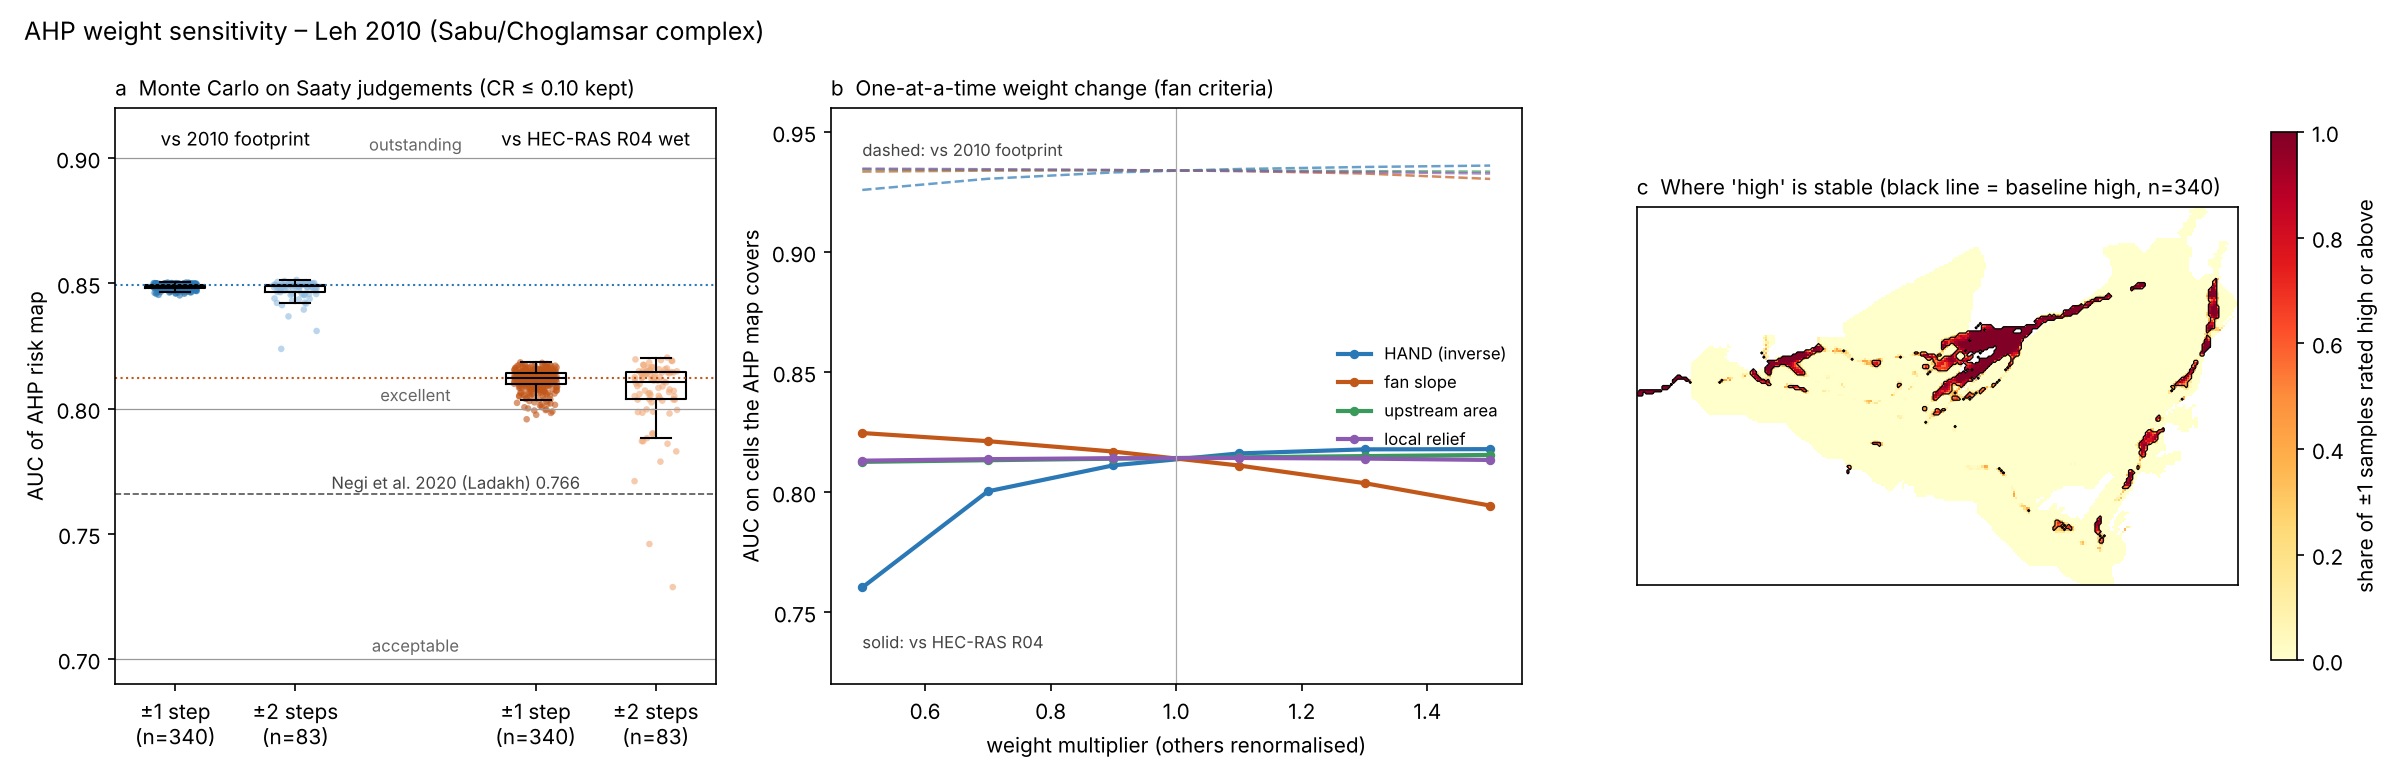
\includegraphics[width=\textwidth]{ahp_sensitivity_2010.png}
  \caption{AHP sensitivity. (a) AUC under random perturbation of the pairwise judgements; (b) one-at-a-time weight changes; (c) share of samples in which each cell stays high or above.}
  \label{fig:sens}
\end{figure*}

\subsection{Who is exposed}
\begin{figure*}[t]
  \centering
  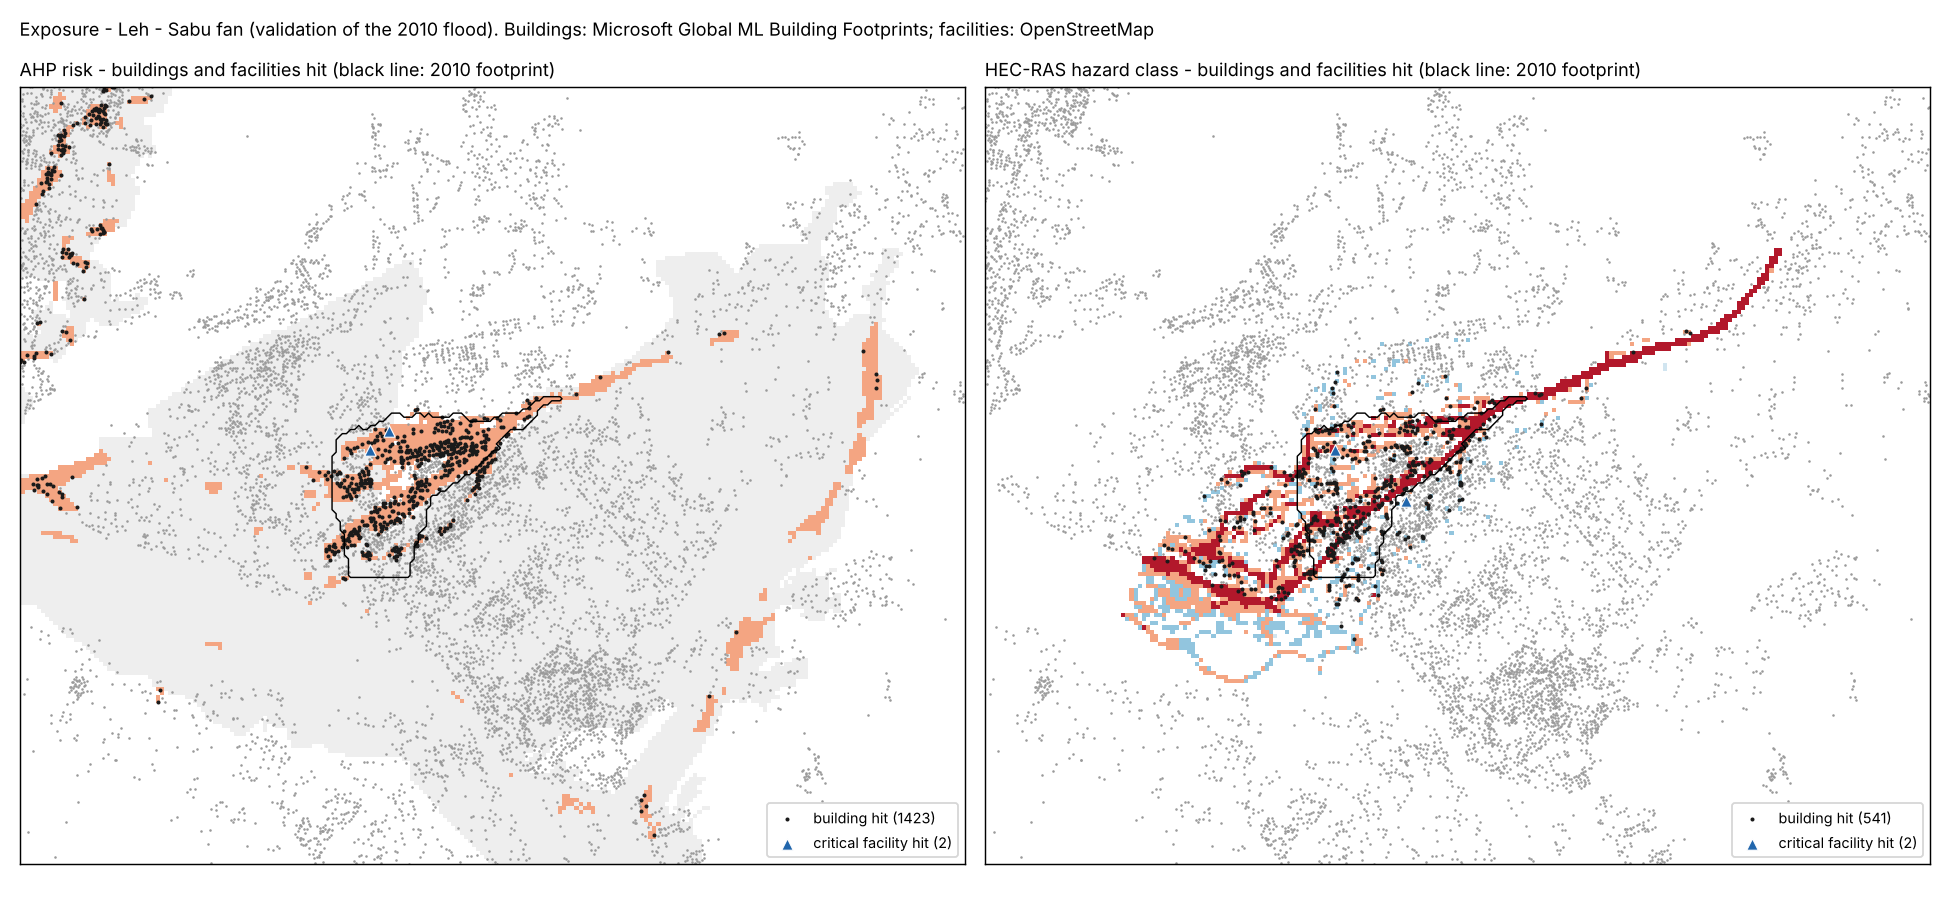
\includegraphics[width=0.85\textwidth]{exposure_map_leh2010.png}
  \caption{Buildings and critical facilities hit, by AHP risk (left) and HEC-RAS hazard class (right); black line: 2010 footprint.}
  \label{fig:exposure}
\end{figure*}
Of 25,384 buildings in the area (Figure~\ref{fig:exposure}):
\begin{itemize}
  \item the AHP map rates 1,423 high or above;
  \item the HEC-RAS hindcast floods 541 to 0.3\,m or more, 200 of them in the extreme class;
  \item 791 present-day buildings lie inside the 2010 footprint.
\end{itemize}
Inside the surveyed window, the AHP map flags 54\% of the buildings that flooded in 2010 at ``high'' (FAR 0.17) and 86\% at ``moderate'' (FAR 0.33). HEC-RAS flags 41\% at 0.3\,m and 78\% at any depth, so much of the 2010 damage was in shallow fringe flow.

The hindcast floods 8.7\,km of road, 3.3\,km of it in the extreme class, and two bridges. Among facilities, the Leh District Jail sits in the extreme class, on a high-risk cell and inside the 2010 footprint. A public school and a fuel station are also exposed.

% =====================================================================================
\section{Transfer Test: Dharali 2025}\label{sec:dharali}
\begin{table}[t]
  \caption{Dharali 2025, default settings of the humid-mountain profile, DEM only, no rainfall. Published values from \cite{kumar2026,isro2025}.}
  \label{tab:dharali}
  \small
  \begin{tabular}{@{}p{0.48\columnwidth}cc@{}}
    \toprule
    Check & \texttt{fanrisk} & Published \\
    \midrule
    Fan found automatically & no & -- \\
    Catchment (one manual apex) & 18.3\,km$^2$ & 17\,km$^2$ \\
    Melton ruggedness & 0.82 & 0.80 \\
    Flow type & debris flow & debris flow \\
    Cells high+, within 250\,m of deposit & 46\% & -- \\
    Fan area; AHP high on it & 13; 4.8\,ha & 18--20\,ha \\
    \bottomrule
  \end{tabular}
\end{table}
With every setting at the default of the humid-mountain profile, the fully automatic run finds no fan (Table~\ref{tab:dharali}). The openness detector assumes that a fan opens onto a wider trunk valley. At Dharali the Bhagirathi is itself a gorge: openness along the Kheer Gad peaks at 7 of 16 directions and closes again at the confluence. Lowering the threshold did not help, because the logic also expects the valley to stay open downstream. We left the detector unchanged and report the failure. An alternative steep-zone detector \cite{norini2016} over-detects here (26 fans, the one on the deposit with its apex 700\,m above the village).

The tool's documented fallback is one manual apex. We placed it where the Khirganga enters the deposition zone mapped by NRSC \cite{nrsc2025}. With it, the pipeline measures the catchment within 8\%, matches the Melton ruggedness (0.82 against 0.80), and so classifies the event as a \emph{debris flow}. The same defaults give a clear-water flood for Leh, which is also correct. Within 250\,m of the deposit, 46\% of cells are high risk or above. The mapped fan (13\,ha) is smaller than the deposit, which crossed to the Bhagirathi.

One published coordinate for Dharali lies about 1.4\,km east of the mapped deposit, so event checks should use mapped extents rather than village points.

% =====================================================================================
\section{Bias Test with HEC-RAS: Kedarnath 2013}\label{sec:kedarnath}
\begin{table}[t]
  \caption{Kedarnath 2013: default settings of the humid-mountain profile, the tool's own SCS hydrograph of 210\,mm in 12\,h, no channel burn. Leh values are the R04 runs of Table~\ref{tab:burn} read back the same way.}
  \label{tab:kedarnath}
  \small
  \begin{tabular}{@{}p{0.44\columnwidth}cc@{}}
    \toprule
    Check & Kedarnath & Leh \\
    \midrule
    Trunk fan found automatically & no & yes \\
    Catchment: apex; town & 18.6; 38.6\,km$^2$ & -- \\
    Melton ruggedness; flow type & 0.72; debris & 0.30; clear \\
    Peak inflow, m$^3$/s (R04; R05) & 109; 199 & 1,070 \\
    Depth; speed in the town & 1.6--2.6\,m; 5--6\,m/s & -- \\
    Wet cells at the model edge & 0 & 0 \\
    Severe cells, AHP high+ & 89\% & -- \\
    AUC, AHP vs HEC-RAS & 0.73--0.75 & 0.83--0.86 \\
    \bottomrule
  \end{tabular}
\end{table}
\begin{figure*}[t]
  \centering
  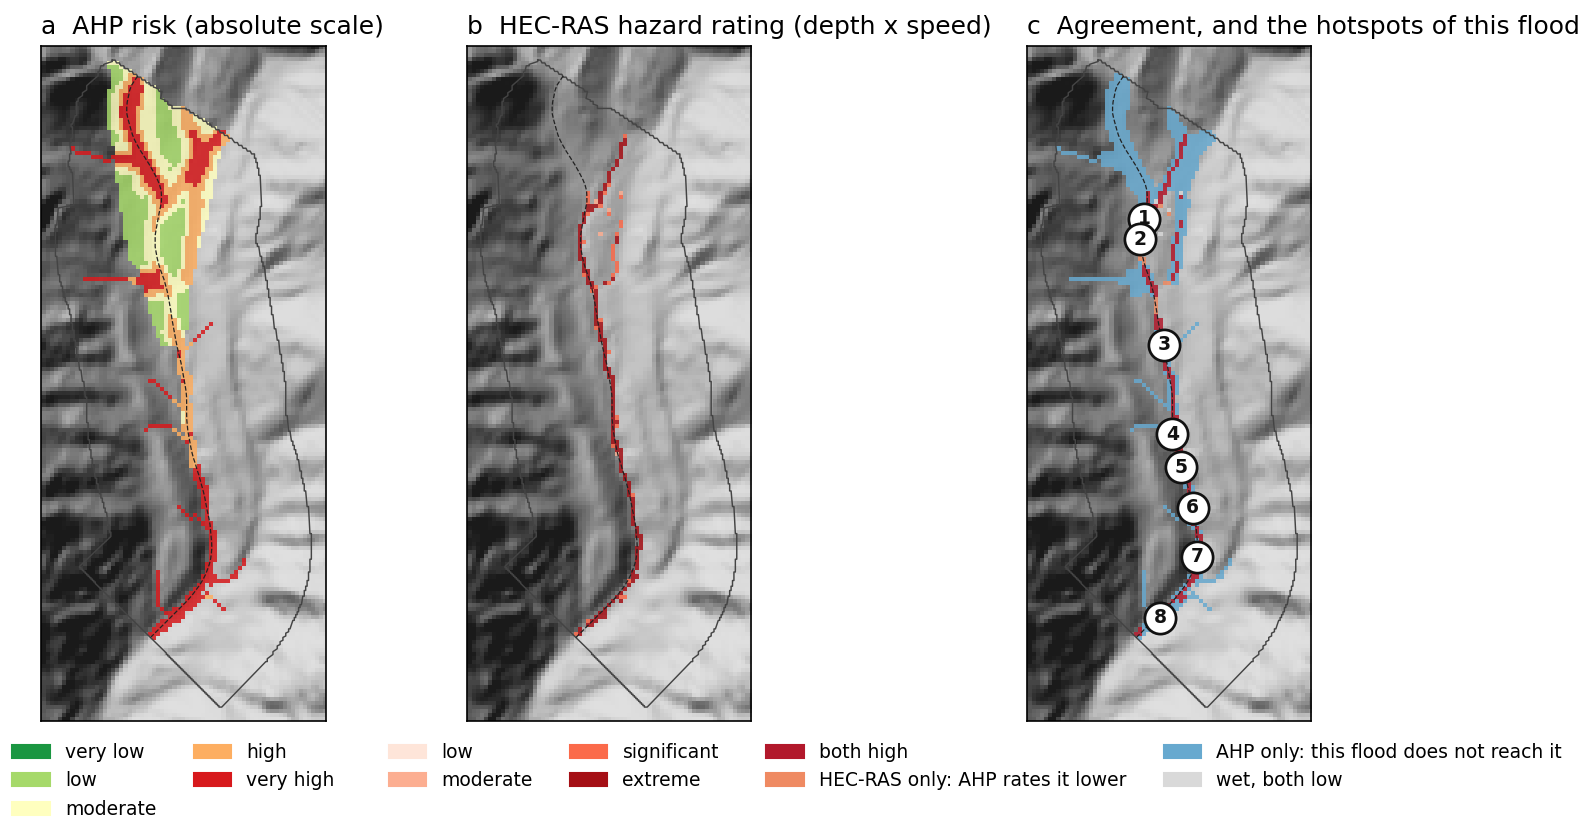
\includegraphics[width=0.86\textwidth]{figures/kedarnath_2013_R04.png}
  \caption{Kedarnath 2013, run R04 (clear water, 109\,m$^3$/s). (a) AHP risk on the Mandakini fan complex. (b) HEC-RAS hazard rating. (c) Agreement; hotspots 1--2 lie in Kedarnath town. Blue cells are high on the AHP map but outside this one feeder's flood. Settings are the tool's defaults; nothing is copied from Leh.}
  \label{fig:kedarnath}
\end{figure*}
The Leh results could hide choices that only work there: the arid profile, the observed hydrograph, the 2\,m channel burn, the reach of the model. We therefore ran the full chain on Kedarnath with none of them (Table~\ref{tab:kedarnath}). The DEM was downloaded fresh; the profile is humid-mountain; the inflow is the tool's SCS hydrograph of the 210\,mm that fell in 12\,h at Chorabari \cite{singh2015}; there is no burn; the reach and width are the defaults; the bundled template was re-fitted to UTM zone 44N (Leh is 43N).

\textbf{Stages 1--2.} As at Dharali, the automatic detector misses the trunk apex (by 1.5\,km) and puts the town on a 3\,km$^2$ side-stream fan; one manual apex on the Mandakini fixes this. The catchment is 18.6\,km$^2$ at the apex and 38.6\,km$^2$ below the Saraswati confluence at the town, and reaches the published 67\,km$^2$ about 5.5\,km downstream. The paper gives no outlet for that figure, so the DEM and the publication agree if the valley is taken to end above Rambara. The Melton ratio of 0.72 gives a debris flow, as observed.

\textbf{Stage 3.} Both runs completed in about 30 minutes each, with a volume error under 0.01\% and no water against the model edge. The flood follows the Mandakini through the town at 1.6--2.6\,m and 5--6\,m/s, extreme on the hazard scale, and reaches the temple point (Figure~\ref{fig:kedarnath}). Of the cells HEC-RAS rates significant or extreme, 89\% are high or very high on the AHP map. The AHP's AUC against the simulated flood is 0.73 (R04) and 0.75 (R05, bulked for debris), lower than the 0.83--0.86 of the Leh runs. Most of the gap is in what the two maps cover. The AHP flags all seven feeders of the complex, including the Saraswati branch that one simulated feeder does not reach. The simulated flood also stays in a channel one or two 29\,m cells wide, so rank correlation with depth is 0.29 against 0.58 at Leh.

\textbf{What the test found.} One step was Leh-specific: the outflow line was lengthened by 900\,m along a single edge of the model outline. At Kedarnath that edge is 333\,m long, and the step failed. It now follows the outline round corners and stops short of the inflow line, and it gives the same result at Leh. No AHP weight, profile setting or HEC-RAS parameter needed changing. The inflow is rain only: the lake outburst is not modelled, so 109--199\,m$^3$/s is a lower bound on 17 June 2013.

% =====================================================================================
\section{Impact Assessment Design}\label{sec:impact}
Accuracy is necessary but not sufficient: the tool only matters if officials read it correctly and change decisions. We designed a three-phase assessment for the next stage, structured by the four early-warning elements \cite{wmo2018}. It has not yet been run.

\textbf{Evaluation questions.}
\begin{enumerate}
  \item Accuracy.
  \item Comprehension.
  \item Better decisions.
  \item Uptake into the District Disaster Management Plan.
  \item Equity and harm. A hazard label can lower land values or be used to move poorer households, and renters, seasonal workers, herders and tourists are easily missed.
\end{enumerate}

\textbf{Phases.}
\begin{itemize}
  \item \textbf{Phase A: usability.} 8--12 DDMA staff, engineers and councillors do five tasks in the web viewer, an 8-item map-reading test, and the System Usability Scale \cite{brooke1996}. The target is a mean of 70 or more, ``good'' on the adjective scale of \cite{bangor2009}.
  \item \textbf{Phase B: tabletop exercise.} 15--25 participants follow the HSEEP format \cite{hseep2020}. Mixed groups draw evacuation zones, road closures and assembly points for a forecast storm, first without the tool and then with it. Each drawn zone is scored against the 2010 footprint with the same CSI used for the maps, so the tool's effect on decisions becomes a number.
  \item \textbf{Phase C: household survey.} About 400 households, stratified by hazard class, plus a comparison fan without outreach for a difference-in-differences design. Questions follow the Protective Action Decision Model \cite{lindell2012}: threat perception, protective-action perception and trust in the source.
\end{itemize}

\textbf{Indicators.} Fourteen indicators run from outputs to impact. Examples are map skill, map-reading score, change in the CSI of drawn zones, households who know their zone and route, adoption in the district plan, permits in extreme zones, and a harm log. Collection and reporting formats are fixed: a ward brief, a facility hazard card, an After-Action Report and a web map with aggregate layers only. The study needs ethics approval at IIT Delhi before fieldwork.

% =====================================================================================
\section{Discussion and Limitations}\label{sec:limits}
\textbf{What the cheap screen is good for.} After the routing fix, the AHP map ranks the 2010 footprint better than the hydraulic model (AUC 0.85 against 0.77) and agrees with it (AUC 0.81). At Kedarnath, with no Leh setting, the agreement is lower (0.73--0.75), but 89\% of the cells the simulation rates significant or extreme are already high on the AHP map. It runs in seconds per DEM, so it can choose where the 2D solver should run next. The hydraulic model adds what the AHP cannot: depths, speeds, hazard classes and a check against a measured section.

\textbf{Limitations.}
\begin{itemize}
  \item The apex detector fails in narrow trunk valleys (Dharali, Kedarnath), and fan outlines there are smaller than deposits.
  \item Lake outbursts are not modelled; at Kedarnath the inflow is rain only, and no observed footprint exists to score it.
  \item A 27--30\,m DEM is as wide as the channel. Finer terrain (Cartosat 10\,m, drone or lidar survey) is not freely available for these valleys; the free ALOS 12.5\,m product is largely resampled 30\,m data.
  \item Several values are fixed judgements and were not perturbed: the scale end-points of Table~\ref{tab:ahp}, the class breaks and the 40\,m burn width. HEC-RAS models one feeder per run.
  \item HEC-RAS runs clear water with one roughness. Bingham debris-flow runs need rheology nobody measured for these sites.
  \item Road embankments and culverts, which diverted the 2010 flow \cite{bhatt2011}, are not in the terrain.
  \item The validation footprint is traced from a published figure (rms 17\,m), and exposure counts use today's buildings, not 2010's.
  \item The 2010 hindcast uses the observed hydrograph. With DEM-derived inputs and uniform rain, the Sabu peak is under-predicted by 61\%, because a cloudburst rains on part of a basin. This is why the pipeline is scenario-driven rather than forecast-driven, as first proposed: a forecast-driven warning needs a cloudburst-scale storm model, not uniform design rain. On the small Leh-town catchment, where the cloudburst covers the whole basin, uniform rain is within 6.5\%.
\end{itemize}

% =====================================================================================
\section{Conclusion}
A freely available DEM is enough to find the fans, rank where flash floods will hurt, build and run a 2D hydraulic model, and list who is exposed, with skill that can be measured against an observed flood. On Leh 2010 the pipeline matches the observed footprint (AUC 0.85 for the AHP screen, 0.77 for HEC-RAS) and the measured depth at Sabu (within 3\%). It is robust to the expert weights and to roughness. On Dharali 2025 it transfers once a single apex is given, and gets the flow type right. On Kedarnath 2013 the whole chain, HEC-RAS included, runs with default settings, and the AHP and the hydraulic model agree on where the flood is most dangerous; the only Leh-specific step we found has been fixed. All code, data and results are open at \url{https://github.com/SaharshLaud/fanrisk}, so a district team or a researcher can repeat every number here and run the same chain on their own valley.

\begin{acks}
We thank Prof. Aaditeshwar Seth for guidance throughout the ICTD course. Building outlines \copyright\ Microsoft (ODbL); roads and facilities \copyright\ OpenStreetMap contributors (ODbL); DEM Copernicus GLO-30 \copyright\ DLR and Airbus, provided under COPERNICUS by the EU and ESA; background imagery \copyright\ Esri, Maxar, Earthstar Geographics.
\end{acks}

\begin{thebibliography}{40}
\bibitem{thayyen2013} R.~J. Thayyen, A.~P. Dimri, P.~Kumar, and G.~Agnihotri. 2013. Study of cloudburst and flash floods around Leh, India, during August 4--6, 2010. \emph{Natural Hazards} 65(3), 2175--2204. doi:10.1007/s11069-012-0464-2.
\bibitem{bhatt2011} C.~M. Bhatt, G.~S. Rao, P.~Manjusree, and V.~Bhanumurthy. 2011. Potential of high resolution satellite data for disaster management: a case study of Leh, Jammu \& Kashmir (India) flash floods, 2010. \emph{Geomatics, Natural Hazards and Risk} 2(4), 365--375. doi:10.1080/19475705.2011.580014.
\bibitem{negi2020} H.~S. Negi et~al. 2020. Susceptibility assessment of rainfall induced debris flow zones in Ladakh--Nubra region, Indian Himalaya. \emph{Journal of Earth System Science} 129, 30.
\bibitem{sharma2023} C.~P. Sharma et~al. 2023. Debris flow susceptibility assessment of Leh Valley, Ladakh, based on concepts of connectivity, propagation and evidence-based probability. \emph{Natural Hazards} 115, 1833--1859.
\bibitem{wilford2004} D.~J. Wilford, M.~E. Sakals, J.~L. Innes, R.~C. Sidle, and W.~A. Bergerud. 2004. Recognition of debris flow, debris flood and flood hazard through watershed morphometrics. \emph{Landslides} 1, 61--66. doi:10.1007/s10346-003-0002-0.
\bibitem{descally2010} F.~A. de~Scally, I.~F. Owens, and J.~Louis. 2010. Controls on fan depositional processes in the schist ranges of the Southern Alps, New Zealand, and implications for debris-flow hazard assessment. \emph{Geomorphology} 122(1--2), 99--116. doi:10.1016/j.geomorph.2010.06.002.
\bibitem{santangelo2012} N.~Santangelo et~al. 2012. Topographic predictors of susceptibility to alluvial fan flooding, Southern Apennines. \emph{Earth Surface Processes and Landforms} 37(8), 803--817. doi:10.1002/esp.3197.
\bibitem{norini2016} G.~Norini, M.~C. Zuluaga, I.~J. Ortiz, D.~T. Aquino, and A.~M.~F. Lagmay. 2016. Delineation of alluvial fans from Digital Elevation Models with a GIS algorithm for the geomorphological mapping of the Earth and Mars. \emph{Geomorphology} 273, 134--149. doi:10.1016/j.geomorph.2016.08.010.
\bibitem{saaty1980} T.~L. Saaty. 1980. \emph{The Analytic Hierarchy Process}. McGraw-Hill.
\bibitem{karkani2021} A.~Karkani et~al. 2021. Flash flood susceptibility evaluation in human-affected areas using geomorphological methods: the case of 9 August 2020, Euboea, Greece. \emph{GeoHazards} 2(4), 366--382.
\bibitem{feizizadeh2014} B.~Feizizadeh and T.~Blaschke. 2014. An uncertainty and sensitivity analysis approach for GIS-based multicriteria landslide susceptibility mapping. \emph{International Journal of Geographical Information Science} 28(3), 610--638. doi:10.1080/13658816.2013.869821.
\bibitem{chen2010} Y.~Chen, J.~Yu, and S.~Khan. 2010. Spatial sensitivity analysis of multi-criteria weights in GIS-based land suitability evaluation. \emph{Environmental Modelling \& Software} 25(12), 1582--1591. doi:10.1016/j.envsoft.2010.06.001.
\bibitem{elsebaie2023} I.~H. Elsebaie, A.~Q. Kawara, and A.~O. Alnahit. 2023. Mapping and assessment of flood risk in the Wadi Al-Lith Basin, Saudi Arabia. \emph{Water} 15(5), 902. doi:10.3390/w15050902.
\bibitem{rascommander} CLB Engineering. 2026. \emph{ras-commander}: HEC-RAS automation library, version 0.113. \url{https://github.com/gpt-cmdr/ras-commander}.
\bibitem{wmo2018} World Meteorological Organization. 2018. \emph{Multi-hazard Early Warning Systems: A Checklist}. WMO, Geneva.
\bibitem{copdem} European Space Agency. Copernicus DEM GLO-30. Registry of Open Data on AWS, \url{https://registry.opendata.aws/copernicus-dem/}.
\bibitem{kumar2026} V.~Kumar, N.~Chauhan, A.~K. Srivastav, Y.~Sundriyal, R.~Sinha, R.~Negi, V.~Gupta, A.~Verma, M.~Puniya, and R.~Devrani. 2026. Dharali debris flow on 5 August 2025, Uttarakhand: event reconstruction and geomorphic implications. \emph{Current Science} 130(3), 229--238. doi:10.18520/cs/v130/i3/229-238.
\bibitem{isro2025} Indian Space Research Organisation. 2025. Indian satellite data based analysis of the Dharali flash flood. \url{https://www.isro.gov.in/ISRO_EN/indian_satellite_data_based_analysis_of_the_dharali_flash_flood.html}.
\bibitem{nrsc2025} National Remote Sensing Centre / NDEM. 2025. Dharali, Uttarkashi: debris deposition map (6 August 2025).
\bibitem{msbuildings} Microsoft. Global ML Building Footprints. \url{https://github.com/microsoft/GlobalMLBuildingFootprints}.
\bibitem{nobre2011} A.~D. Nobre et~al. 2011. Height Above the Nearest Drainage: a hydrologically relevant new terrain model. \emph{Journal of Hydrology} 404, 13--29.
\bibitem{holmgren1994} P.~Holmgren. 1994. Multiple flow direction algorithms for runoff modelling in grid based elevation models: an empirical evaluation. \emph{Hydrological Processes} 8(4), 327--334.
\bibitem{fd2321} Defra and Environment Agency. 2006. \emph{Flood Risks to People, Phase 2}. R\&D Technical Report FD2321/TR1.
\bibitem{chow1988} V.~T. Chow, D.~R. Maidment, and L.~W. Mays. 1988. \emph{Applied Hydrology}. McGraw-Hill.
\bibitem{kirpich1940} Z.~P. Kirpich. 1940. Time of concentration of small agricultural watersheds. \emph{Civil Engineering} 10(6), 362.
\bibitem{obrien1988} J.~S. O'Brien and P.~Y. Julien. 1988. Laboratory analysis of mudflow properties. \emph{Journal of Hydraulic Engineering} 114(8), 877--887.
\bibitem{riley1999} S.~J. Riley, S.~D. DeGloria, and R.~Elliot. 1999. A terrain ruggedness index that quantifies topographic heterogeneity. \emph{Intermountain Journal of Sciences} 5(1--4), 23--27.
\bibitem{chow1959} V.~T. Chow. 1959. \emph{Open-Channel Hydraulics}. McGraw-Hill.
\bibitem{jarrett1984} R.~D. Jarrett. 1984. Hydraulics of high-gradient streams. \emph{Journal of Hydraulic Engineering} 110(11), 1519--1539.
\bibitem{hosmer2013} D.~W. Hosmer, S.~Lemeshow, and R.~X. Sturdivant. 2013. \emph{Applied Logistic Regression} (3rd ed.). Wiley.
\bibitem{brooke1996} J.~Brooke. 1996. SUS: a ``quick and dirty'' usability scale. In \emph{Usability Evaluation in Industry}. Taylor \& Francis, 189--194.
\bibitem{bangor2009} A.~Bangor, P.~Kortum, and J.~Miller. 2009. Determining what individual SUS scores mean: adding an adjective rating scale. \emph{Journal of Usability Studies} 4(3), 114--123.
\bibitem{hseep2020} FEMA. 2020. \emph{Homeland Security Exercise and Evaluation Program (HSEEP)}. U.S. Department of Homeland Security.
\bibitem{singh2015} D.~S. Singh et al. 2015. Brief communication: Rapid assessment of the 2013 Kedarnath disaster. \emph{Natural Hazards and Earth System Sciences} 15, 1597--1601. doi:10.5194/nhess-15-1597-2015.
\bibitem{lindell2012} M.~K. Lindell and R.~W. Perry. 2012. The Protective Action Decision Model: theoretical modifications and additional evidence. \emph{Risk Analysis} 32(4), 616--632. doi:10.1111/j.1539-6924.2011.01647.x.
\end{thebibliography}

\end{document}
